% Type of the document
\documentclass{beamer}
% elementary packages:
\usepackage{graphicx}
\usepackage[latin1]{inputenc}
\usepackage[T1]{fontenc}
\usepackage[english]{babel}
\usepackage{listings}
\usepackage{xcolor}
\usepackage{eso-pic}
\usepackage{mathrsfs}
\usepackage{url}
\usepackage{amssymb}
\usepackage{amsmath}
\usepackage{multirow}
\usepackage{hyperref}
\usepackage{booktabs}
\usepackage{tikz}

% additional packages
\usepackage{bbm}
\usetheme{Boadilla}

% packages supplied with ise-beamer:
\usepackage{cooltooltips}
\usepackage{colordef}
\usepackage{beamerdefs}
\usepackage{lvblisting}

% Change the pictures here:
% logobig and logosmall are the internal names for the pictures: do not modify them. 
% Pictures must be supplied as JPEG, PNG or, to be preferred, PDF
\pgfdeclareimage[height=2cm]{logobig}{hulogo}
% Supply the correct logo for your class and change the file name to "logo". The logo will appear in the lower
% right corner:
\pgfdeclareimage[height=0.7cm]{logosmall}{logo}


% Title page outline:
% use this number to modify the scaling of the headline on title page
\renewcommand{\titlescale}{0.9}
% the title page has two columns, the following two values determine the percentage each one should get
\renewcommand{\titlescale}{.9}
\renewcommand{\leftcol}{0.6}



% Define the title.Don't forget to insert an abbreviation instead 
% of "title for footer". It will appear in the lower left corner:
\title[SPL WS2017/18 - Labour Force Participation in Europe]{Labour Force Participation of the Elderly 
in Europe  - The importance of being healthy}


% Define the authors:
\authora{Phi Nguyen} % a-c
\authorb{Julian Winkel}
\authorc{Claudia Guenther}

% Define any internet addresses, if you want to display them on the title page:
\def\linka{}
\def\linkb{}
\def\linkc{}
\vspace{2cm}
% Define the institute:
\institute{Statistical Programming Languages \\
WS2017/2018
 \\

Ladislaus von Bortkiewicz Chair of Statistics \\
Humboldt--Universit�t zu Berlin \\}



% Comment the following command, if you don't want, that the pdf file starts in full screen mode:
\hypersetup{pdfpagemode=FullScreen}

%Start of the document
\begin{document}

% create the title slide, layout controlled in beamerdefs.sty and the foregoing specifications
\frame[plain]{
\titlepage
}

% The titles of the different sections of you talk, can be included via the \section command. The title will be displayed in the upper left corner. To indicate a new section, repeat the \section command with, of course, another section title
%%%%%%%%%%%%%%%%%%%%%%%%%%%%%%%%%%%%%%%%%%%%%%%%%%%%%%%%%%%%%%%%%%%%%%%%%%%%%%%%%%%%%%%%%%%%%%%%%%%%%%%%%%%%%%%%%%%%%%%%
\section{random}
%%%%%%%%%%%%%%%%%%%%%%%%%%%%%%%%%%%%%%%%%%%%%%%%%%%%%%%%%%%%%%%%%%%%%%%%%%%%%%%%%%%%%%%%%%%%%%%%%%%%%%%%%%%%%%%%%%%%%%%%

% (A numbering of the slides can be useful for corrections, especially if you are
% dealing with large tex-files)
%%%%%%%%%%%%%%%%%%%%%%%%%%%%%%%%%%%%%%%%%%%%%%%%%%%%%%%%%%%%%%%%%%%%%%%%%%%%%%%%%%%%%%%%%%%%%%%%%%%%%%%%%%%%%%%%%%%%%%%

%%%%%%%%%%%%%%%%%%%%%%%%%%%%%%%%%%%%%%%%%%%%%%%%%%%%%%%%%%%%%%%%%%%%%%%%%%%%%%%%%%%%%%%%%%%%%%%%%%%%%%%%%%%%%%%%%%%%%%%%
% No number on outline slide
\section{}
\useheadtemplate{%
    \raisebox{-0.75cm}{\parbox{\textwidth}{%
            \footnotesize{\color{isegray}%
                \insertsection\ \leavevmode\leaders\hrule height3.2pt depth-2.8pt\hfill\kern0pt\ }}}
}

\frame{
\frametitle{Outline}
\begin{enumerate}
\item Motivation
\item Background \& Methods
\item Current project status\
\begin{center}
\begin{tabular}{ll}
 \hspace{-4.5cm}
 Overview on quantlets\\
   \hspace{-4.5cm}
  Highlights
\end{tabular}
\end{center}
\item Next steps

\end{enumerate}
}

% No number on outline slide
\useheadtemplate{%
    \raisebox{-0.75cm}{\parbox{\textwidth}{%
            \footnotesize{\color{isegray}%
                \insertsection\ \leavevmode\leaders\hrule height3.2pt depth-2.8pt\hfill\kern0pt\ \thesection-\thepage}}}}
\setcounter{section}{1}

%%%%%%%%%%%%%%%%%%%%%%%%%%%%%%%%%%%%%%%%%%%%%%%%%%%%%%%%%%%%%%%%%%%%%%%%%%%%%%%%%%%%%%%%%%%%%%%%%%%%%%%%%%%%%%%%%%%%%%%%
\section{Motivation}
%%%%%%%%%%%%%%%%%%%%%%%%%%%%%%%%%%%%%%%%%%%%%%%%%%%%%%%%%%%%%%%%%%%%%%%%%%%%%%%%%%%%%%%%%%%%%%%%%%%%%%%%%%%%%%%%%%%%%%%%

% Subsections are not visible on the actual slide, but are displayed as bookmarks in the pdf file. Their application facilitates an easy navigation trough large pdf files.
%%%%%%%%%%%%%%%%%%%%%%%%%%%%%%%%%%%%%%%%%%%%%%%%%%%%%%%%%%%%%%%%%%%%%%%%%%%%%%%%%%%%%%%%%%%%%%%%%%%%%%%%%%%%%%%%%%%%%%%%
\subsection{General ideas}
%%%%%%%%%%%%%%%%%%%%%%%%%%%%%%%%%%%%%%%%%%%%%%%%%%%%%%%%%%%%%%%%%%%%%%%%%%%%%%%%%%%%%%%%%%%%%%%%%%%%%%%%%%%%%%%%%%%%%%%%

%%%%%%%%%%%%%%%%%%%%%%%%%%%%%%%%%%%%%%%%%%%%%%%%%%%%%%%%%%%%%%%%%%%%%%%%%%%%%%%%%%%%%%%%%%%%%%%%%%%%%%%%%%%%%%%%%%%%%%%%
\frame{
\frametitle{Labour Force Participation of Elderly in Europe}
\begin{itemize}
\item Changing demographics in Europe: Social, health \& economic challenge 
\begin{itemize}
\item  Policy \&  employment implications
\end{itemize}
\item SHARE panel database of micro data on health, socio-economic status and social and family networks 
\begin{itemize}
\item 120,000 individuals (50+), 27 participating countries
\item easySHARE as simplified data set
\end{itemize}

\end{itemize}
 
\begin{figure}[htb]
		
\includegraphics[scale=0.3]{Figures/easySHARE}	
\end{figure}	
\begin{center}
available on \href{http://www.share-project.org/special-data-sets/easyshare.html}{http://www.share-project.org/}
\end{center}

}



%%%%%%%%%%%%%%%%%%%%%%%%%%%%%%%%%%%%%%%%%%%%%%%%%%%%%%%%%%%%%%%%%%%%%%%%%%%%%%%%%%%%%%%%%%%%%%%%%%%%%%%%%%%%%%%%%%%%%%%%

\section{Background \& Methods}
\frame[containsverbatim]{
\frametitle{Background and Methods for Quantlets}
Adriaan Kalwij and Frederic Vermeulen (2005), IZA DP No. 1887 \\
\newblock{\em 
Labour Force Participation of the Elderly
in Europe: The Importance of Being Healthy} \\
\newblock 
\begin{itemize}
\item How is the labor force participation behavior of individuals aged 50-64 in 11 European countries influenced by different health indicators?
\item Investigate employment potential of healthy elderly Europeans
\begin{center}
\begin{tabular}{ll}
  Cross-sectional probit regression model (ML estimation) \\
  Marginal effect at means \& Wald tests \\
  Counterfactual excercise \\
  Lack of graphical representation
  \end{tabular}
\end{center}
\end{itemize}

}

%%%%%%%%%%%%%%%%%%%%%%%%%%%%%%%%%%%%%%%%%%%%%%%%%%%%%%%%%%%%%%%%%%%%%%%%%%%%%%%%%%%%%%%%%%%%%%%%%%%%%%%%%%%%%%%%%%%%%%%%
\section{Current project status}


\frame[containsverbatim]{
\frametitle{Overview on Quantlets}
\begin{itemize}
\item Quantlet 1: Read and Clean easyshare dataset
\item Quantlet 2: Summary Statistics
\item         Quantlet 3: Probit Regression
\item Quantlet 4: Wald Test
\item         Quantlet 5: Counterfactual exercise
 \item        Quantlet 6: Graphical representation
\end{itemize} 
}


%%%%%%%%%%%%%%%%%%%%%%%%%%%%%%%%%%%%%%%%%%%%%%%%%%%%%%%%%%%%%%%%%%%%%%%%%%%%%%%%%%%%%%%%%%%%%%%%%%%%%%%%%%%%%%%%%%%%%%%%
\frame[containsverbatim]{
\frametitle{Quantlet 1: Read and Clean easyshare dataset}
\begin{itemize}
\item Input: Data frame and wave. Output: List of data frames
\item Imputation of missing values
\item Conversion of country data from ISO code to a human-readable format 
\item Relevant error messages
\end{itemize} 


\begin{columns}
\begin{column}{0.95\textwidth}
\begin{lstlisting}
# Split data frames into country/gender splits, then standardize numeric

splits    = split(df.out, f = list(df.out$country, 
df.out$gender), drop = TRUE)
df.reg    = standardize.df(df.out)
df.splits = lapply(splits, standardize.df)

\end{lstlisting}
\end{column}
\end{columns}

}

%%%%%%%%%%%%%%%%%%%%%%%%%%%%%%%%%%%%%%%%%%%%%%%%%%%%%%%%%%%%%%%%%%%%%%%%%%%%%%%%%%%%%%%%%%%%%%%%%%%%%%%%%%%%%%%%%%%%%%%%



\frame[containsverbatim]{
\frametitle{Quantlet 1: Read and Clean easyshare dataset}

\begin{columns}
\begin{column}{0.95\textwidth}
\begin{lstlisting}
# Create necessary dummary variables for regression

dummify = function(data.frame) {
        data.frame = data.frame %>%
            dplyr::select(-country, -gender)       
        model      = ~ 0 + .                       
        new.df     = model.matrix(model, data.frame)
        new.df     = data.frame(new.df)
        return(new.df) 
    }
    
df.splits = lapply(df.splits, dummify) 

\end{lstlisting}
\href{https://github.com/phister/SPL_Project/blob/master/Scripts/ReadAndClean.R}{\quantnet}
\end{column}
\end{columns}
}




%%%%%%%%%%%%%%%%%%%%%%%%%%%%%%%%%%%%%%%%%%%%%%%%%%%%%%%%%%%%%%%%%%%%%%%%%%%%%%%%%%%%%%%%%%%%%%%%%%%%%%%%%%%%%%%%%%%%%%%%
\frame[containsverbatim]{
\frametitle{Quantlet 2: Summary Statistics}
\begin{itemize}
\item Summary statistic tables of health characteristics of the elderly
\item contains functions that calculate labor participation rates and type of labor chosen by gender and country
\item Usage of `pmap` in `purrr` package to loop over groupings
\item Prints tables into readable html format

\end{itemize} 
\href{https://github.com/phister/SPL_Project/blob/master/Scripts/SummaryStatistics.R}{\quantnet}


}
%%%%%%%%%%%%%%%%%%%%%%%%%%%%%%%%%%%%%%%%%%%%%%%%%%%%%%%%%%%%%%

\frame[containsverbatim]{
\frametitle{Quantlet 2: Summary Statistics}

\begin{figure}[htb]
	\begin{center}
	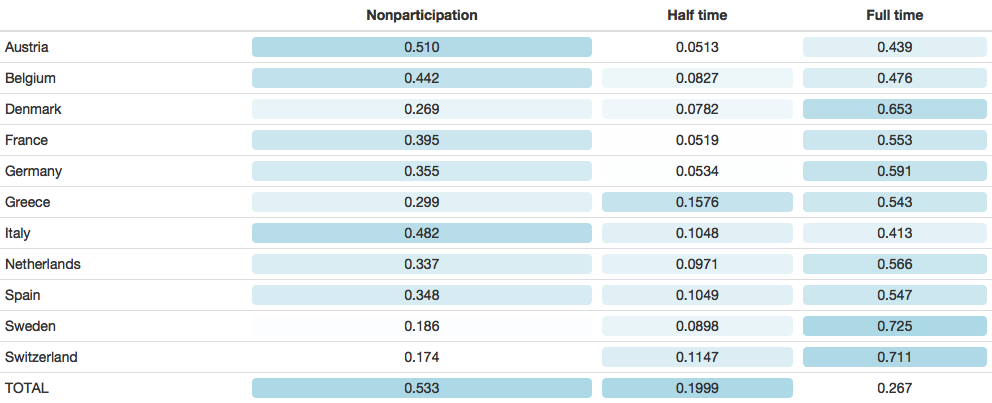
\includegraphics[scale=0.35]{Figures/df6}	\end{center}
\end{figure}


}

%%%%%%%%%%%%%%%%%%%%%%%%%%%%%%%%%%%%%%%%%%%%%%%%%%%%%%%%%%



%%%%%%%%%%%%%%%%%%%%%%%%%%%%%%%%%%%%%%%%%%%%%%%%%%%%%%%%%%%%%%%%%%%%%%%%%%%%%%%%%%%%%%%%%%%%%%%%%%%%%%%%%%%%%%%%%%%%%%%%
\frame[containsverbatim]{
\frametitle{Quantlet 3: Probit Regression}
\begin{itemize}
\item Probit regression for each country and both gender groups based on  `glm` 
\item Calculation of marginal effects based on `probitmfx`
\item Wald test using own-built Wald test

\end{itemize} 
\href{https://github.com/phister/SPL_Project/blob/master/Scripts/ProbitRegression.R}{\quantnet}


\begin{columns}
\begin{column}{0.95\textwidth}
\begin{lstlisting}

allModels = lapply(df.splits, function(z){
           z = z[-z$age50] 
       model = glm(z$labor_participationTRUE ~., 
      family = binomial(link = "probit"), data = z)
return(model)
 })
 
allSummaries = lapply(allModels, summary)


\end{lstlisting}
\href{https://github.com/phister/SPL_Project/blob/master/Scripts/ProbitRegression.R}{\quantnet}
\end{column}
\end{columns}


}
%%%%%%%%%%%%%%%%%%%%%%%%%%%%%%%%%%%%%%%%%%%%%%%%%%%%%%%%%%%%%%
\frame[containsverbatim]{
\frametitle{Quantlet 3: Probit Regression}
\begin{columns}
\begin{column}{1.0\textwidth}
\begin{lstlisting}
wald.log = list() 
for(i in 1:length(allSummaries)){
  SummaryElement = allSummaries[[i]]
  health = c(16:19)
  testOutput = try(joint.wald.test(allSummaries[[i]], health, 0.95))
  
  if(class(testOutput) == "try-error"){
    
    msg = paste0("Wald Test failed for Model Element ", i)
    warning(msg)
    wald.log[[i]] = "Error"  
  } else{   
    wald.log[[i]] = testOutput  
  }}


\end{lstlisting}
\href{https://github.com/phister/SPL_Project/blob/master/Scripts/ProbitRegression.R}{\quantnet}
\end{column}
\end{columns}


}
%%%%%%%%%%%%%%%%%%%%%%%%%%%%%%%%%%%%%%%%%%%%%%%%%%%%%%%%%%%%%%
%%%%%%%%%%%%%%%%%%%%%%%%%%%%%%%%%%%%%%%%%%%%%%%%%%%%%%%%%%%%%%
\frame[containsverbatim]{
\frametitle{Quantlet 4: Wald Test}
\begin{itemize}
\item Wald test for joint significance of regression coefficients
\end{itemize} 
\href{https://github.com/phister/SPL_Project/blob/master/Scripts/LoadWald.R}{\quantnet}
\vspace{-0.3cm}
\begin{columns}
\begin{column}{1.0\textwidth}
\begin{lstlisting}
joint.wald.test = function(model.summary, spec, signf.l){
    
joint.wald.test        = numeric(6)
names(joint.wald.test) = c("Name","W","p-value", "df")
beta                   = model.summary$coefficients[,1]
Var_beta_est           = vcov(model.summary)
W = t(beta[spec]) %*% solve(Var_beta_est[spec,spec]) %*% beta[spec]

    chi2               = qchisq(signf.l, df=length(spec))
    pval               = 1-pchisq(W,length(spec))
    joint.wald.test[1] = "Chi2 test"
    joint.wald.test[2] = format(   W, digits = 4)

\end{lstlisting}
\end{column}
\end{columns}



}

%%%%%%%%%%%%%%%%%%%%%%%%%%%%%%%%%%%%%%%%%%%%%%%%%%%%%%%%%%
%%%%%%%%%%%%%%%%%%%%%%%%%%%%%%%%%%%%%%%%%%%%%%%%%%%%%%%%%%%%%%
\frame[containsverbatim]{
\frametitle{Quantlet 5: Counterfactual exercise}
\begin{itemize}
\item Estimation of current and counterfactual employment rate
\item Definition of data set with perfectly healthy individuals
\item Calculate decline in participation due to decline in health condition

\end{itemize} 
\href{https://github.com/phister/SPL_Project/blob/master/Scripts/Counterfactual.R}{\quantnet}

\begin{columns}
\begin{column}{1.0\textwidth}
\begin{lstlisting}
X.cf   = function(model){
     X                   = model$data
     X_cf                = X
     X_min               = data.frame(t(apply(X, 2, min)))
     names.vec           = c("h_chronic", "h_adlaTRUE", "h_obeseTRUE")
     X_cf[, names.vec]  = X_min[names.vec]
  \end{lstlisting}
\end{column}
\end{columns}


}

%%%%%%%%%%%%%%%%%%%%%%%%%%%%%%%%%%%%%%%%%%%%%%%%%%%%%%%%%%%%%%%%%%%%%%%%%%%%%%%%%%%%%%%%%%%%%%%%%%%%%%%%%%%%%%%%%%%%%%%%%
\frame[containsverbatim]{
\frametitle{Quantlet 6: Graphical representation}
\begin{columns}
\begin{column}{1.0\textwidth}
\begin{figure}[htb]
	\begin{center}
	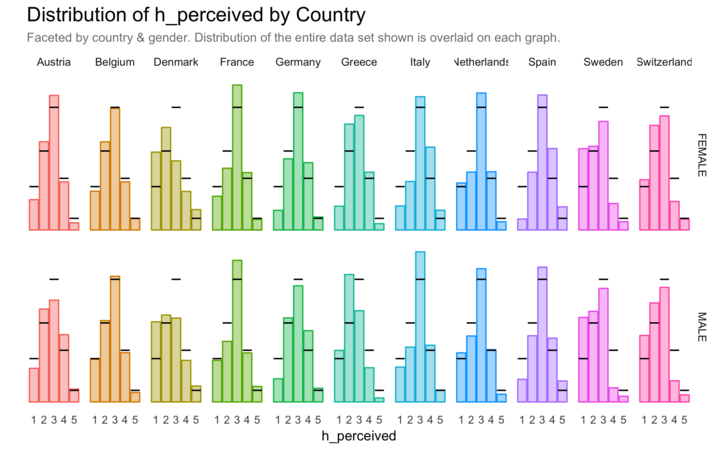
\includegraphics[scale=0.38]{Figures/health}	\end{center}

\end{figure}
\href{https://github.com/phister/SPL_Project/blob/master/Scripts/Graphics.R}{\quantnet}
\end{column}
\end{columns}

}

%%%%%%%%%%%%%%%%%%%%%%%%%%%%%%%%%%%%%%%%%%%%%%%%%%%%%%%%%%%%%%%

%%%%%%%%%%%%%%%%%%%%%%%%%%%%%%%%%%%%%%%%%%%%%%%%%%%%%%%%%%%%%%%%%%%%%%%%%%%%%%%%%%%%%%%%%%%%%%%%%%%%%%%%%%%%%%%%%%%%%%%%
\section{Next steps}
%%%%%%%%%%%%%%%%%%%%%%%%%%%%%%%%%%%%%%%%%%%%%%%%%%%%%%%%%%%%%%%%%%%%%%%%%%%%%%%%%%%%%%%%%%%%%%%%%%%%%%%%%%%%%%%%%%%%%%%%

%%%%%%%%%%%%%%%%%%%%%%%%%%%%%%%%%%%%%%%%%%%%%%%%%%%%%%%%%%%%%%%%%%%%%%%%%%%%%%%%%%%%%%%%%%%%%%%%%%%%%%%%%%%%%%%%%%%%%%%%
\frame[containsverbatim]{
\frametitle{Next steps for project}

\begin{itemize}
\item Add additional graphics (choropleth maps)
\item Add error messages to Wald tests
\item Export all replicated results
\item Review code to assure coherence with style guide
\item Review code to assure coherence between quantlets

\end{itemize}
	\href{https://github.com/phister/SPL_Project}{\quantnet}

}

%%%%%%%%%%%%%%%%%%%%%%%%%%%%%%%%%%%%%%%%%%%%%%%%%%%%%%%%%%%%%%%%%%%%%%%%%%%%%%%%%%%%%%%%%%%%%%%%%%%%%%%%%%%%%%%%%%%%%%%%
%%%%%%%%%%%%%%%%%%%%%%%%%%%%%%%%%%%%%%%%%%%%%%%%%%%%%%%%%%%%%%%%%%%%%%%%%%%%%%%%%%%%%%%%%%%%%%%%%%%%%%%%%%%%%%%%%%%%%%%%

% Define the end of the document:
\end{document}
